\documentclass[12pt,a4paper]{report}
%\usepackage[english]{babel}
\usepackage[utf8]{inputenc}
\usepackage{amsmath}
\usepackage{amsfonts}
\usepackage{amssymb}
\usepackage{makeidx}
\usepackage{graphicx}
\usepackage{setspace}
\usepackage{times}
\usepackage{float}
\usepackage{subfigure}
\usepackage{subfiles}
\usepackage{longtable}
\usepackage{enumitem}
\usepackage{pdfpages}
\usepackage{pdfpages}
%\usepackage{}
%\usepackage[skip=12pt,font=footnotesize]{caption}
\graphicspath{./images/}
%%%BibLatex % % % % % % % % % % % % % % % % % % % 

\usepackage[style=ieee, backend=bibtex,style=numeric, sorting=none]{biblatex}
\addbibresource{ref.bib}
%\usepackage[superscript,biblabel]{cite}
\AtBeginDocument{\renewcommand{\bibname}{References}}
\makeatletter
%\renewcommand{\bibfont}{\small}
%\renewcommand{\bibname}{References}
\newrobustcmd*{\nobibliography}{%
	\@ifnextchar[%]
	{\blx@nobibliography}
	{\blx@nobibliography[]}}
\def\blx@nobibliography[#1]{}
\appto{\skip@preamble}{\let\printbibliography\nobibliography}
\makeatother


\DeclareCiteCommand{\supercite}[\mkbibsuperscript]
{\iffieldundef{prenote}
	{}
	{\BibliographyWarning{Ignoring prenote argument}}%
	\iffieldundef{postnote}
	{}
	{\BibliographyWarning{Ignoring postnote argument}}}
{\usebibmacro{citeindex}%
	\bibopenbracket\usebibmacro{cite}\bibclosebracket}
{\supercitedelim}
{}

\let\cite=\supercite
%\usepackage[superscript]{cite}
% % % % % % % % % % % % % % % % % % % % % % % % % %



% % % % % % % % % % % % % % % % % % % % % % % % % % 
\title{Bibliography management: \texttt{biblatex} package}
\usepackage[left=38mm,right=25.4mm,top=25.4mm,bottom=25.4mm]{geometry}
\usepackage{fancyhdr}
\pagestyle{fancy}
\rhead{\leftmark}
\lhead{130320702512}
\lfoot{}
%\setcounter{page}{1}
\rfoot{}
\chead{}
\cfoot{\thepage}
%\renewcommand{\headrulewidth}{0.4pt}
%\renewcommand{\footrulewidth}{0.4pt}

%\usepackage[skip=12pt,font=footnotesize]{caption}

%\makeatletter
%\renewcommand{\@dotsep}{10000} 
%\makeatother

%\pagestyle{fancy}
%\fancyhead{}
%\fancyhead[R]{\leftmark }
%\fancyfoot{}
%\fancyfoot[LE,RO]{\thepage}
%\fancyfoot[LO,CE]{ }


\renewcommand{\headrulewidth}{1pt}
\renewcommand{\footrulewidth}{1pt}
\usepackage{setspace}
\renewcommand{\baselinestretch}{1.5}
%\setlength{\parindent}{2 em}
%\renewcommand{\baselinestretch}{1.50}\normalsize
\renewcommand*\contentsname{Table of Content}

\author{Shivang Patel}
\title{ADB Practicals}

\begin{document}

\begin{enumerate}
% % % % % % % % % % % % % % % % % % % % % % % % % % % % % % % % % % % % %
% % SCHEMA % % % % % % % % % % % % % % % % % % % % % % % % % % % % % % %
% % % % % % % % % % % % % % % % % % % % % % % % % % % % % % % % % % % % %
	\item{ \fontsize{14}{12} \textbf{Schema for the Practicals :} }{
		
		\paragraph{}{
			The overall design of the database is called the database schema. A database schema corresponds to
			the variable declarations (along with associated type definitions) in a program. Each
			variable has a particular value at a given instant. The values of the variables in a
			program at a point in time correspond to an instance of a database schema.
			}
		\paragraph{}{
			Here, for the practicals, we are using schema for Banking Enterprise. This schema shown in below figure...
			
			\begin{figure}[H]
				\centering
				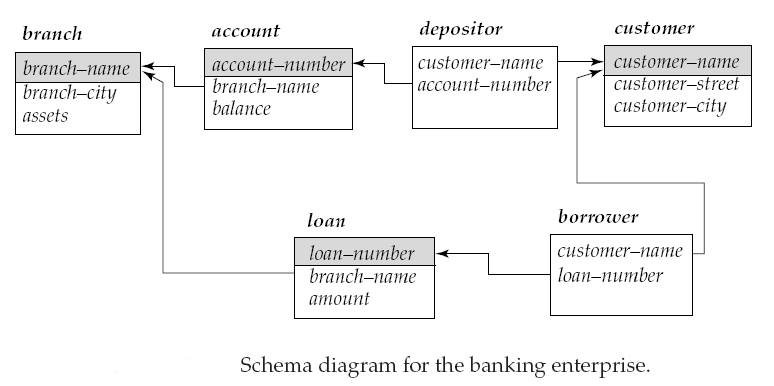
\includegraphics[scale=.5]{./images/schema}
				\caption{Banking Enterprise - A Schema}
			\end{figure}
			
			}	
		
		}
\end{enumerate}		
	\clearpage
	\newpage

\begin{enumerate}	
	
	% % % % % % % % % % % % % % % % % % % % % % % % % % % % % % % % % % %
	% % P1 % % % % % % % % % % % % % % % % % % % % % % % % % % % % % %
	% % % % % % % % % % % % % % % % % % % % % % % % % % % % % % % % % % %
	\item{\nonumber \fontsize{14}{12} \textbf{Aim : To perform various SQL commands with logical Operators and Predicates.} }{
		\newline
		\textbf{Logical Operator : }		
		There are three Logical Operators namely, AND, OR, and NOT. These operators compare two conditions at a time to determine whether a row can be selected for the output. When retrieving data using a SELECT statement, you can use logical operators in the WHERE clause, which allows you to combine more than one condition.\\
		\textbf{"OR" Logical Operator : }
		If you want to select rows that satisfy at least one of the given conditions, you can use the logical operator, OR.
		\textbf{Syntax :}
		\begin{verbatim}
			SELECT C1,C2,...,Cn
			FROM TABEL_NAME
			WHERE <condition> OR <condition>
			;
		\end{verbatim} 
		Here, in below figure show implemented "OR Logical Operator".
		\begin{figure}[H]
			\centering
			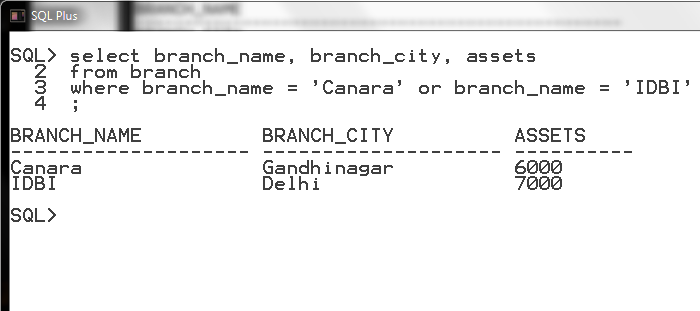
\includegraphics[scale=.55]{./images/prac1_or2}
			\caption{Logical Operator : OR}
		\end{figure}
				 
		\textbf{"AND" Logical Operator : }
		If you want to select rows that must satisfy all the given conditions, you can use the logical operator, AND. 
		}
		\textbf{Syntax :}		
		\begin{verbatim}
		SELECT C1,C2,...,Cn
		FROM TABEL_NAME
		WHERE <condition> AND <condition>
		;
		\end{verbatim}
		Here, in below figure show implemented "AND Logical Operator".
		\begin{figure}[H]
			\centering
			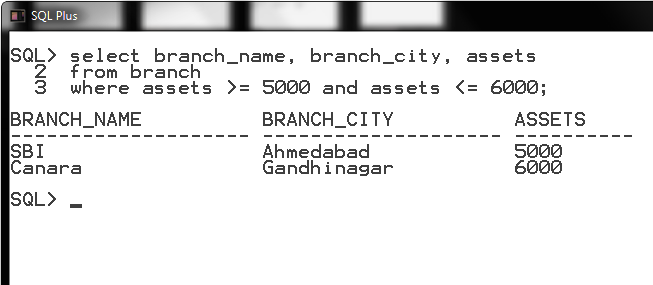
\includegraphics[scale=.55]{./images/prac1_and2}
			\caption{Logical Operator : AND}
		\end{figure}		
		
		\textbf{"NOT" Logical Operator:}
		If you want to find rows that do not satisfy a condition, you can use the logical operator, NOT. NOT results in the reverse of a condition. That is, if a condition is satisfied, then the row is not returned. 
		\textbf{Syntax :}		
		\begin{verbatim}
		SELECT C1,C2,...,Cn
		FROM TABEL_NAME
		WHERE <condition> NOT <condition>
		;
		\end{verbatim}		
		Here, in below figure show implemented "NOT Logical Operator".
		\begin{figure}[H]
			\centering
			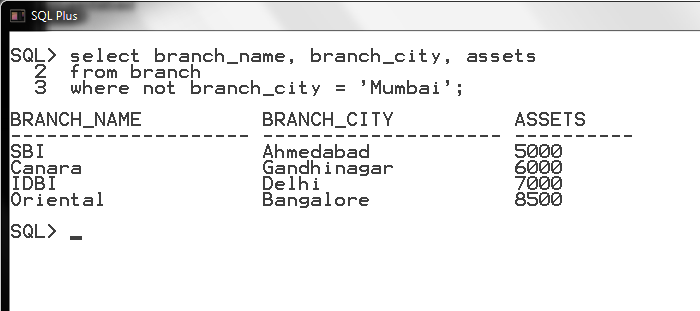
\includegraphics[scale=.55]{./images/prac1_not2}
			\caption{Logical Operator : NOT}
		\end{figure}		
		
		\textbf{SQL Predicates : }
		There are other comparison keywords available in sql which are used to enhance the search capabilities of a sql query. They are "WHERE","IN", "BETWEEN...AND", "IS NULL", "LIKE”...etc.\\
		Here, in below figure show implemented "WHERE predicate". 
		\begin{figure}[H]
			\centering
			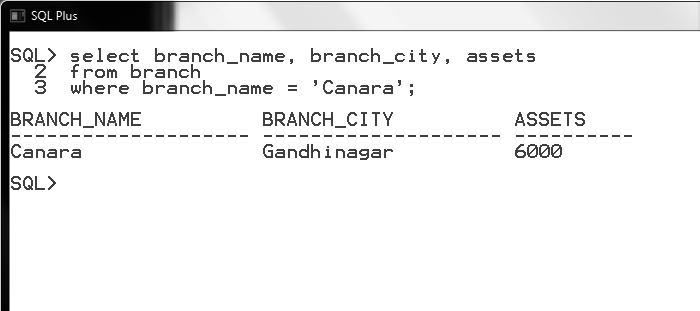
\includegraphics[scale=.55]{./images/prac1_predicate2}
			\caption{Predicate : WHERE}
		\end{figure}
	\clearpage
	\newpage	
	
	% % % % % % % % % % % % % % % % % % % % % % % % % % % % % % % % % % %
	% % P2 % % % % % % % % % % % % % % % % % % % % % % % % % % % % % %
	% % % % % % % % % % % % % % % % % % % % % % % % % % % % % % % % % %	
	\item{ \fontsize{14}{12} \textbf{To Perform various Data Constraint with table level and column level specifications.} }{
		
		Constraints are the rules enforced on data columns on table. These are used to limit the type of data that can go into a table. This ensures the accuracy and reliability of the data in the database.\\
		
		Constraints could be \textbf{column level} or \textbf{table level}. Column level constraints are applied only to one column, whereas table level constraints are applied to the whole table.\\
		
		List of Constraints :
		\begin{itemize}
			\item Primary Key
			\item Foreign Key
			\item Unique Key
			\item Null Value
		\end{itemize}
		
		On the next page, we show the Primary Key constraint syntax at column level and table level with it's demo.
		
		\newpage 
		\textbf{Syntax : Primary Key at table level}
		\begin{verbatim}
			PRIMARY KEY ( <ColumName>,...,<ColumName> )
		\end{verbatim}
		\begin{figure}[H]
			\centering
			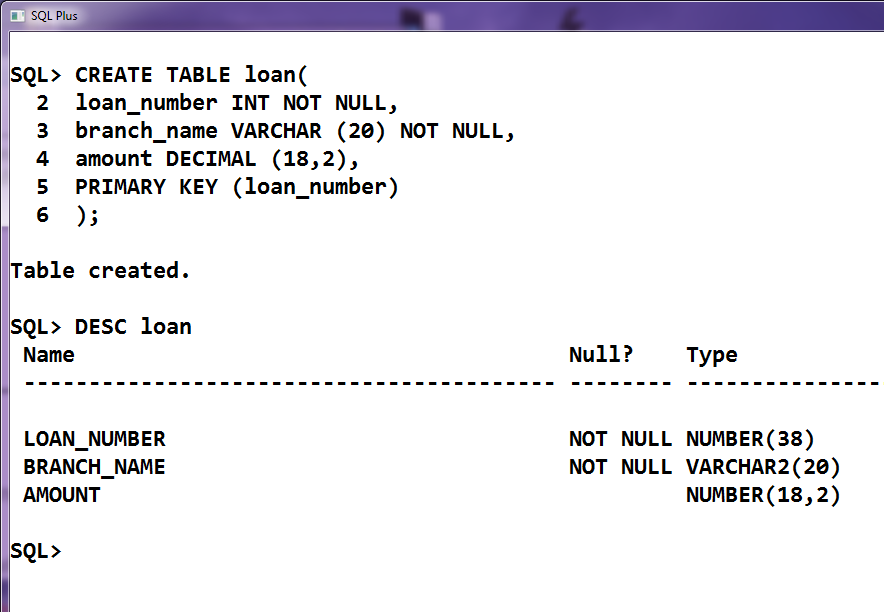
\includegraphics[scale=.45]{./images/2_table_level_primery_key_constraints}
			\caption{Constraint at Table Level : PRIMARY KEY}
		\end{figure}
				
		\textbf{Syntax : Primary Key at column level}
		\begin{verbatim}
			<ColumName> <Datatype>(<size>) PRIMARY KEY		
		\end{verbatim}				
		\begin{figure}[H]
			\centering
			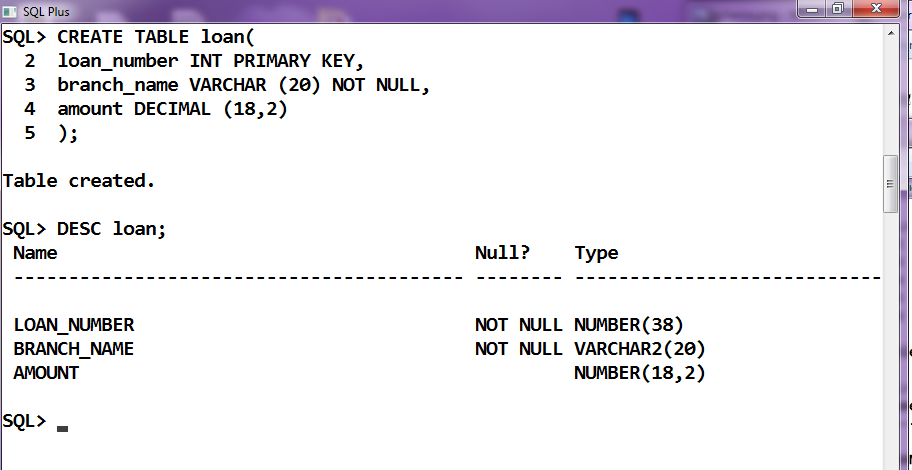
\includegraphics[scale=.45]{./images/2_columan_level_primery_key_constraints}
			\caption{Constraint at Column Level : PRIMARY KEY}
		\end{figure}
				
		}	
	\clearpage
	\newpage	

	% % % % % % % % % % % % % % % % % % % % % % % % % % % % % % % % % % %
	% % P3 % % % % % % % % % % % % % % % % % % % % % % % % % % % % % %
	% % % % % % % % % % % % % % % % % % % % % % % % % % % % % % % % % % %
	\item{ \fontsize{14}{12} \textbf{To perform the concept of Grouping Data from tables in SQL.} }{
		The SQL GROUP BY clause is used in collaboration with the SELECT statement to arrange identical data into groups.
		\textbf{Syntax : GROUP BY Clause}
		\begin{verbatim}
			SELECT <column1>,<column2>,...,<columnN>,
				FUNCTION(<Expration>)
				FROM TABLE_NAME
				WHERE <Condition>
				GROUP BY <column1>,<column2>,...,<columnN>
				Other Clause
				; 
		\end{verbatim}
		
		\textbf{Explanation : }Here, in the demo we are grouping the customer name, whose account number like '10x' and customer have more then 1 account. First figure show the depositor table and second figure show the result of successful grouping. 				
		\begin{figure}[H]
			\centering
			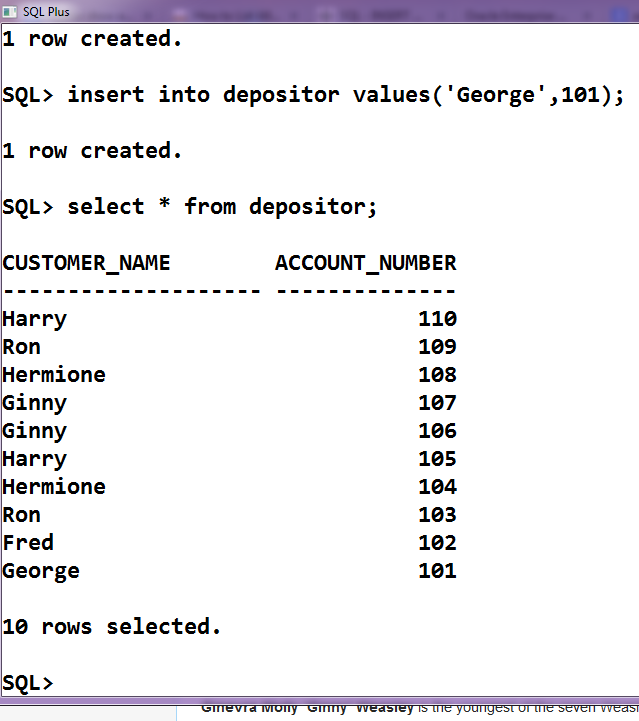
\includegraphics[scale=.45]{./images/3_1_table3_insert1}
			\caption{Show the 'depositor' Table}
		\end{figure}
		\begin{figure}[H]
			\centering
			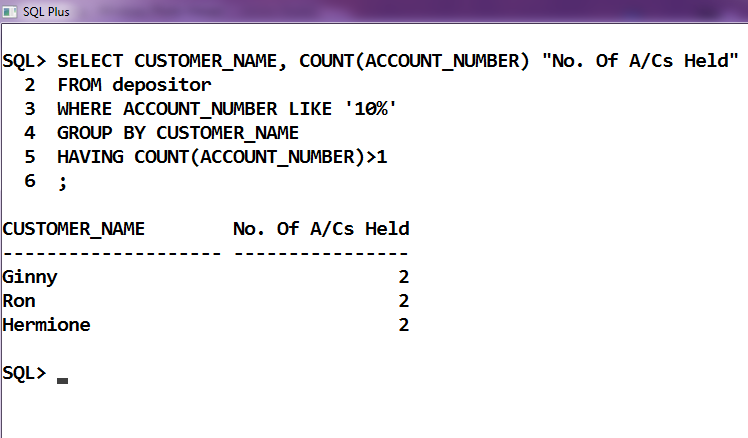
\includegraphics[scale=.45]{./images/3_2_table3_groupBy_HavingClause}
			\caption{Show the Result of Grouping}
		\end{figure}				
		}
	\clearpage
	\newpage	

	% % % % % % % % % % % % % % % % % % % % % % % % % % % % % % % % % % %
	% % P4 % % % % % % % % % % % % % % % % % % % % % % % % % % % % % %
	% % % % % % % % % % % % % % % % % % % % % % % % % % % % % % % % % % %
	\item{ \fontsize{14}{12} \textbf{To perform various types of join.} }{
		The SQL Joins clause is used to combine records from two or more tables in a database. A JOIN is a means for combining fields from two tables by using values common to each. Here, it is noticeable that the join is performed in the WHERE clause. Several operators can be used to join tables, such as $ = $, $ < $, $ > $, $ <> $, $ <= $, $ >= $, $ != $, BETWEEN, LIKE, and NOT; they can all be used to join tables. However, the most common operator is the equal symbol.
		}
	\clearpage
	\newpage	

	% % % % % % % % % % % % % % % % % % % % % % % % % % % % % % % % % % %
	% % P5 % % % % % % % % % % % % % % % % % % % % % % % % % % % % % %
	% % % % % % % % % % % % % % % % % % % % % % % % % % % % % % % % % % %
	\item{ \fontsize{14}{12} \textbf{Implementation of Indexes and Sequences.} }	
	\clearpage
	\newpage

	% % % % % % % % % % % % % % % % % % % % % % % % % % % % % % % % % % %
	% % P6 % % % % % % % % % % % % % % % % % % % % % % % % % % % % % %
	% % % % % % % % % % % % % % % % % % % % % % % % % % % % % % % % % % %
	\item{ \fontsize{14}{12} \textbf{Implementation of view.} }	
	\clearpage
	\newpage

	% % % % % % % % % % % % % % % % % % % % % % % % % % % % % % % % % % %
	% % P7 % % % % % % % % % % % % % % % % % % % % % % % % % % % % % %
	% % % % % % % % % % % % % % % % % % % % % % % % % % % % % % % % % % %
	\item{ \fontsize{14}{12} \textbf{Implementation of PL/SQL block.} }	
	\clearpage
	\newpage

	% % % % % % % % % % % % % % % % % % % % % % % % % % % % % % % % % % %
	% % P8 % % % % % % % % % % % % % % % % % % % % % % % % % % % % % %
	% % % % % % % % % % % % % % % % % % % % % % % % % % % % % % % % % % %
	\item{ \fontsize{14}{12} \textbf{To Perform Various Transaction Control Commands.} }	
	\clearpage
	\newpage

	% % % % % % % % % % % % % % % % % % % % % % % % % % % % % % % % % % %
	% % P9 % % % % % % % % % % % % % % % % % % % % % % % % % % % % % %
	% % % % % % % % % % % % % % % % % % % % % % % % % % % % % % % % % % %
	\item{ \fontsize{14}{12} \textbf{Implementation of cursor.} }{
		\begin{enumerate}
			\item{ \fontsize{14}{12} \textbf{Implicit cursor.}}
			\item{ \fontsize{14}{12} \textbf{Explicit cursor.}}			
		\end{enumerate}
		}
	\clearpage
	\newpage	
		
	% % % % % % % % % % % % % % % % % % % % % % % % % % % % % % % % % % %
	% % P10 % % % % % % % % % % % % % % % % % % % % % % % % % % % % % %
	% % % % % % % % % % % % % % % % % % % % % % % % % % % % % % % % % %	
	\item{ \fontsize{14}{12} \textbf{Implementation of concurrency control with the help of locking mechanisms.} }{
		\begin{enumerate}
			\item{ \fontsize{14}{12} \textbf{Implicit and explicit lock using SQL.}}
			\item{ \fontsize{14}{12} \textbf{Explicit locking using PL/SQL.}}			
			\item{ \fontsize{14}{12} \textbf{Implementation of Deadlock.}}						
		\end{enumerate}
	}
	\clearpage
	\newpage
	
	% % % % % % % % % % % % % % % % % % % % % % % % % % % % % % % % % % %
	% % P11 % % % % % % % % % % % % % % % % % % % % % % % % % % % % % %
	% % % % % % % % % % % % % % % % % % % % % % % % % % % % % % % % % %	
	\item{ \fontsize{14}{12} \textbf{To perform Error handling in PL/SQL.} }					
	\clearpage
	\newpage
	
	% % % % % % % % % % % % % % % % % % % % % % % % % % % % % % % % % % %
	% % P12 % % % % % % % % % % % % % % % % % % % % % % % % % % % % % %
	% % % % % % % % % % % % % % % % % % % % % % % % % % % % % % % % % 	
	\item{ \fontsize{14}{12} \textbf{Implementation of Stored Procedure and Function.} }						
	\clearpage
	\newpage

	% % % % % % % % % % % % % % % % % % % % % % % % % % % % % % % % % % %
	% % P13 % % % % % % % % % % % % % % % % % % % % % % % % % % % % % %
	% % % % % % % % % % % % % % % % % % % % % % % % % % % % % % % % % %	
	\item{ \fontsize{14}{12} \textbf{Implementation of Oracle Package.} }		
	\clearpage
	\newpage				
	
	% % % % % % % % % % % % % % % % % % % % % % % % % % % % % % % % % % %
	% % P14 % % % % % % % % % % % % % % % % % % % % % % % % % % % % % %
	% % % % % % % % % % % % % % % % % % % % % % % % % % % % % % % % % %		
	\item{ \fontsize{14}{12} \textbf{Implementation of overloading Procedures and Functions.} }	
	\clearpage
	\newpage
	
	% % % % % % % % % % % % % % % % % % % % % % % % % % % % % % % % % % %
	% % P15 % % % % % % % % % % % % % % % % % % % % % % % % % % % % % %
	% % % % % % % % % % % % % % % % % % % % % % % % % % % % % % % % % %		
	\item{ \fontsize{14}{12} \textbf{Implementation of Trigger.} }{
		\begin{enumerate}
			\item{ \fontsize{14}{12} \textbf{Row Trigger}}
			\item{ \fontsize{14}{12} \textbf{Statement Trigger}}			
			\item{ \fontsize{14}{12} \textbf{Trigger with Exception}}						
		\end{enumerate}
	}
	\clearpage
	\newpage							
	
\end{enumerate}	
	
\end{document}
